%----------------------------------------------------------------------------------------
%	PREÁMBULO
%----------------------------------------------------------------------------------------

\documentclass[11pt, oneside]{book}
\usepackage[paperwidth=17cm, paperheight=22.5cm, bottom=2.5cm, right=2.5cm]{geometry}

% El borde inferior puede parecerles muy amplio a la vista. Les recomiendo hacer una prueba de impresión antes para ajustarlo

\usepackage{amssymb,amsmath,amsthm} % Símbolos matemáticos
\usepackage[english]{babel}
\usepackage[utf8]{inputenc} % Acentos y otros símbolos 
\usepackage{enumerate}
\PassOptionsToPackage{hyphens}{url}\usepackage{hyperref} % Hipervínculos en el índice
\usepackage{graphicx}
%\usepackage{subfig} % Subfiguras
\graphicspath{{Imagenes/}} % En qué carpeta están las imágenes

% Para eliminar guiones y justificar texto
\tolerance=1
\emergencystretch=\maxdimen
\hyphenpenalty=10000
\hbadness=10000

\linespread{1.25} % Asemeja el interlineado 1.5 de Word

\let\oldfootnote\footnote % Deja espacio entre el número del pie de página y el inicio del texto
\renewcommand\footnote[1]{%
\oldfootnote{\hspace{0.05mm}#1}}

\renewcommand{\thefootnote} {\textcolor{Black}{\arabic{footnote}}} % Súperindice a color negro

\setlength{\footnotesep}{0.75\baselineskip} % Espaciado entre notas al pie

\usepackage{fnpos} % Footnotes al final de pág.

\usepackage[justification=centering, font=bf, labelsep=period, skip=5pt]{caption} % Centrar captions de tablas y ponerlas en negritas

\newcommand{\imagesource}[1]{{\footnotesize Fuente: #1}}

\usepackage{tabularx} % Big tables
\usepackage{graphicx}
\usepackage{adjustbox}
%\usepackage{longtable}

\usepackage{float} % Float tables

%% my comands JESUS LOPEZ
\usepackage{amsfonts}
\usepackage{dcolumn} % for stargazer
\usepackage{longtable} % for split table into pages
%\usepackage{xcolor} % for color in text
\usepackage{booktabs} % for extrakable
\usepackage{makecell} % for extrakable
\usepackage[flushleft]{threeparttable} % for large notes in tables
\usepackage{multirow} % idem
\usepackage{placeins } % to place tablesunder subsection headers
%\usepackage[bottom,splitrule,perpage]{footmisc}
%\usepackage{floatfoot} % The floatrow package offers the \floatfoot macro for notes in addition to a float's \caption
\counterwithout{footnote}{page} % for continuing footnotes numbering 
\usepackage{etoolbox}
\usepackage{booktabs}

\usepackage{hyperref} % to include urls
%\hypersetup{
%    colorlinks=true,
%    linkcolor=blue,
%    filecolor=magenta,      
%    urlcolor=blue,
%    pdfpagemode=FullScreen,
%    citecolor = blue
%    }
    
\usepackage{caption}
\usepackage{subcaption} % to include subfigures
\usepackage{natbib} % to include references




\newcommand\fnote[1]{\captionsetup{font=footnotesize}\caption*{#1}} 

\newcommand{\sym}[1]{#1}
%\AtBeginEnvironment{tabular}{\doublespacing}



%% 


\usepackage[usenames,dvipsnames]{xcolor} % Color

\usepackage{pgfplots} % Gráficas
\pgfplotsset{compat=newest}
\pgfplotsset{width=7.5cm}
\pgfkeys{/pgf/number format/1000 sep={}}

\begin{document}

%----------------------------------------------------------------------------------------
%	PASTA
%----------------------------------------------------------------------------------------

\title{La elasticidad de la tasa de interés de la demanda de crédito: evidencia empírica de empresas mexicanas.} % Con este nombre se guardará el proyecto en writeLaTex

\begin{titlepage}
\begin{center}

\textsc{\Large Instituto Tecnológico Autónomo de México}\\[2em]

%Figura
\begin{figure}[h]
\begin{center}

\includegraphics[scale=0.50]{itam_logo.png}
\end{center}
\end{figure}

% Pueden modificar el tamaño del logo cambiando la escala

\textbf{\LARGE La elasticidad de la tasa de interés de la demanda de crédito: evidencia empírica de empresas mexicanas.}\\[2em]

\textsc{\large Tesis}\\[1em]

\textsc{\large que para obtener el grado de}\\[1em]

\textsc{\LARGE Maestro en Teoría Económica }\\[1em]

\textsc{\large Presenta}\\[1em]

\textsc{\LARGE Jesús López Pérez}\\[1em]


\end{center}

\vspace*{\fill}
\textsc{Ciudad de México \hspace*{\fill} 2023}

\end{titlepage}


%----------------------------------------------------------------------------------------
%	PORTADA
%----------------------------------------------------------------------------------------


\begin{titlepage}
\begin{center}

\textsc{\Large Instituto Tecnológico Autónomo de México}\\[2em]

%Figura
\begin{figure}[h]
\begin{center}

\includegraphics[scale=0.50]{itam_logo.png}
\end{center}
\end{figure}

% Pueden modificar el tamaño del logo cambiando la escala

\textbf{\LARGE La elasticidad de la tasa de interés de la demanda de crédito: evidencia empírica de empresas mexicanas.}\\[2em]

\textsc{\large Tesis}\\[1em]

\textsc{\large que para obtener el grado de}\\[1em]

\textsc{\LARGE Maestro en Teoría Económica }\\[1em]

\textsc{\large Presenta}\\[1em]

\textsc{\LARGE Jesús López Pérez}\\[1em]

\textsc{\large Asesor}\\[1em]

\textsc{\LARGE Dr. José Francisco Tudón Maldonado}\\[2em]

% Asegúrense de escribir el nombre completo de su asesor

\end{center}

\vspace*{\fill}
\textsc{Ciudad de México \hspace*{\fill} 2023}

\end{titlepage}

%----------------------------------------------------------------------------------------
%	DECLARACIÓN
%----------------------------------------------------------------------------------------

\thispagestyle{empty}

\vspace*{\fill}
\begingroup

\noindent
«Con fundamento en los artículos 21 y 27 de la Ley Federal del Derecho de Autor y como titular de los derechos moral y patrimonial de la obra titulada ``\textbf{La elasticidad de la tasa de interés de la demanda de crédito: evidencia empírica de empresas mexicanas.}'', otorgo de manera gratuita y permanente al Instituto Tecnológico Autónomo de México y a la Biblioteca Raúl Bailléres Jr., la autorización para que fijen la obra en cualquier medio, incluido el electrónico, y la divulguen entre sus usuarios, profesores, estudiantes o terceras personas, sin que pueda percibir por tal divulgación una contraprestación.»

% Asegúrense de cambiar el título de su tesis en el párrafo anterior

\centering 

\vspace{5em}

%\rule[1em]{20em}{0.5pt} % Línea para la fecha

\textsc{Jesús López Pérez}
 
\vspace{5em}

\rule[1em]{20em}{0.5pt} % Línea para la firma

\textsc{Fecha}

\vspace{5em}
\rule[1em]{20em}{0.5pt} % Línea para la firma

\textsc{Firma}


\endgroup
\vspace*{\fill}

%----------------------------------------------------------------------------------------
%	DEDICATORIA
%----------------------------------------------------------------------------------------

\pagestyle{plain}
\frontmatter

\chapter*{}
\begin{flushright}
\noindent \textit{Le dedico esta tesis a toda mi familia.}
\end{flushright}



%----------------------------------------------------------------------------------------
%	AGRADECIMIENTOS
%----------------------------------------------------------------------------------------

\section*{Agradecimientos}
\noindent A Dios, por no soltarme de tu mano en todos estos años. A Valeria, sin tu amor no podríamos estar escribiendo esta historia. A Julia Inés y Elías, por enseñarme tanto, a su corta edad. A papá y mamá, por su caminar incansable, les debo todo. A Cris, Nacho y Anabell, por los recuerdos entrañables que construimos en la infancia, y que nos han permitido mantenernos juntos, en la distancia. A Doña Loi, por aceptarme como parte de su gran familia.  A Fran, por tu amistad y apoyo para continuar mis estudios; por enseñarme a apreciar la cotidianeidad. A José Tudón, por su asesoría en esta tesis y por ser guía y apoyo para continuar con mis estudios doctorales. A mis sinodales, Felipe Brugués y Francisco Garrido, sus comentarios fueron muy valiosos para mejorar esta tesis; como siempre, todos los errores son totalmente mi responsabilidad. A mis recomendadores Víctor Guerrero y Carlos Urrutia, por creer en mí. A todos mis profesores en el ITAM, por acercarme cada vez más a la economía. A los amigos de toda la vida que conocí en Cholula, Monterrey, y Ciudad de México; en particular a los compañeros del ITAM, por formar parte de este viaje. Por último, y no menos importante, a las maestras de Gimy Guarderías.

% Esta sección es lo único que la gente lee. True story :)
%----------------------------------------------------------------------------------------
%	RESUMEN
%----------------------------------------------------------------------------------------

\section*{Resumen}

\noindent En esta investigación realizo una estimación de la elasticidad tasa de interés de la demanda de crédito en México utilizando información a nivel de microdatos para pequeñas y medianas empresas. Creo una nueva base de datos de créditos de empresas a partir de datos administrativos. Primero, agrego datos a nivel industria para crear un panel de datos de abril de 2016 a diciembre de 2021, enseguida, utilizo esta base en un modelo de panel con variables instrumentales para mitigar el problema de endogeneidad y el sesgo de variables omitidas. Además, incorporo efectos fijos a nivel de industria, banco, año e industria-año. Los resultados indican que la elasticidad es de $-1.43$, por lo tanto aportan evidencia de una demanda elástica.

\pagestyle{plain}


\noindent 

%----------------------------------------------------------------------------------------
%	TABLA DE CONTENIDOS
%---------------------------------------------------------------------------------------

\tableofcontents

%----------------------------------------------------------------------------------------
%	ÍNDICE DE CUADROS Y FIGURAS
%---------------------------------------------------------------------------------------

\listoftables

\listoffigures

%----------------------------------------------------------------------------------------
%	TESIS
%----------------------------------------------------------------------------------------

\newpage
\noindent 

%----------------------------------------------------------------------------------------
%	Summary
%----------------------------------------------------------------------------------------

\section*{Summary}

\noindent In this investigation, I estimate the interest rate elasticity of credit demand in Mexico using micro-data level information for small and medium size enterprises. I build a novel database of commercial loans from administrative data. I first aggregate the data to the industry-level to create a panel dataset from April 2016 to December 2021, next, I use this database in a panel model with instrumental variables to circumvent the endogeneity and omitted variables problem. Additionally, I incorporate fixed effects at the industry, bank, year, and industry-year level. The results indicate that the elasticity is $-1.43$, indicating an elastic demand. 

\pagestyle{plain}


\mainmatter % Empieza la numeración de las páginas

\pagestyle{plain}

% Incluye los capítulos en el fólder de capítulos


\chapter{Introduction}

Several factors affect the demand for credit. In this paper, I focus on one particular aspect: the choice of how much debt firms incur, thus I provide reasonable estimates of the interest rate elasticity of commercial credit. The magnitude of this elasticity has important implications for policy-relevant questions in several areas of the economy. For example, in recent years the leading party in the Mexican congress has expressed its concerns aimed at regulating the financial sector\footnote{See for instance  \cite{noauthor_monreal_2020} or  \cite{noauthor_ricardo_nodate}.}. These measures include implementing controls on the gap between active and passive interest rates in consumer loans, to limit the amount of fees collected on financial services, and, more recently, to ensure that Small and Medium Enterprises (SMEs\footnote{Defined as those with net annual sales less than 106 million pesos, CNBV.}) have access to cheap loans\footnote{\cite{ceo_monreal_2022}.}; all these in an effort to reduce the banks' profits and in the interest of benefiting society. Regarding the latter, although a specific bill outlining the intended reform has not been made public, we can think of scenarios if the average interest rate is lowered and anticipate the corresponding increase in the amount of credit. 

Credit access is influenced by various factors related to the firm, including its size, age, sector, country of activity, changes in financial indicators, and private signals like economic outlook and credit reputation \citep{Antonecchia2023}. Also, firms demand credit mainly to meet their  start-up, cash flow (meeting financial requirements, general business activities) and investment needs (acquiring new equipment innovation, expansion projects) \citep{OECDnewapproaches2015}. 

The demand for credit is also influenced by the heterogeneity of firms' expectations regarding the business cycle phase, leading to increased accessibility of credit and rising debt levels during economic booms \citep{NBERw20038}. As expansions increase financial institutions' expectations about companies' future revenue improve, thus these positive conditions may facilitate the repayment of loans; similarly, fear of recessions increases fear of potential losses due to defaults and leads to tightening  lending standards.

Changes in the composition of economic sectors in the economy are also relevant for the demand for credit. There is heterogeneity in finance needs by sectors; for instance, usually tertiary sectors demand more credit than primary or secondary, thus, the transition of economies towards a tertiary sector certainly would affect the aggregated demand for credit \citep{chavarin2023importance}.

New technologies and the availability of new means of production that generate more revenue in an industry may boost the development of specific sectors, so firms within them are prone to ask for credit to be early adopters. In this sense, tight credit conditions may hinder firms' investments, weakening productivity, but resource reallocation from low to high-productivity firms can partially offset this impact \citep{azevedo_bank_2021}.

On the other hand, banks and financial institutions grant credit to firms based on their assessment of their risk profile. Financial intermediaries would set prices to reflect known risks and demand would match supply at that price. However, the efficient allocation of credit through interest rates presupposes that information about borrowers' projects is freely available \citep{blundell1992credit}.

This thesis aims to develop an econometric model specifically tailored for estimating the interest-rate elasticity of Mexican companies’ demand for credit. To do so, I exploit panel-level data with firm fixed effects and controls to address potential issues such as omitted variables --related to the factors just mentioned above that are not observed in the data-- and endogeneity --the fact that interest rate and loan amount are jointly determined by the intersection of supply and demand curves-- ; by considering these particularities, the model enhances the robustness of the analysis and strengthens the validity of the findings. 

The main contribution of this research is to show that with minimal data on firm loans, properly handled, and by using appropriate econometric methods, interest rate elasticities can be estimated under a reduced form model of credit demand. To shed light on credit demand, I contribute also to the usage of the National Banking and Stock Commission's (\textit{Comisión Nacional Bancaria y de Valores}, CNBV) publicly available administrative records\footnote{As discussed below, this source of information has been used in the past by other researchers, but they have usually had access to more detailed privately--disclosed data.}$^,$\footnote{The codes used to webscrap the data are available on \url{https://github.com/SrChucho/rc04-data}.}.

This research speaks to the literature of empirical industrial organization to model financial markets. For instance,  \cite{crawford2018asymmetric} uses loan-level firm data from Italy, to evaluate the impact of asymmetric information and imperfect competition. Similarly, \cite{IOANNIDOU202293} consider asymmetric information issues, and employ credit registry data to construct a structural model that sheds light on the importance of collateral for lending; mitigates adverse selection and moral hazard. \cite{benetton2021leverage} considers the impact of leverage deregulation through capital requirements on interest rates. Moreover, \cite{liu2022low} analyzes how interest rates and market power impact productivity growth; they conclude that lower interest rates reduce aggregate investment in productivity growth. While papers such as these can provide insight into the behaviour of the economic agents in the lending process, they often rely on more detailed, usually privately, datasets to address more specific questions.  

To this regard, the results of the structural model of \cite{IOANNIDOU202293} are larger than the one I found here; in a very similar setting, they find that one percentage point increase in interest rate decreases the loan amount demanded at most in  -3.2\% whereas I found -1.4\%. That is, with a more simple, reduced-form model, I can achieve results in the same line, although much smaller. %Nevertheless, I acknowledge that the scope of this research is more limited. 
This is also related to an empirical literature in the banking industry, that studies the role of credit in the economy from the demand (see \cite{dick2008demand}, \cite{beck2012gets}) and the supply side (\cite{branzoli2021role}).

This paper is also related to a literature that studies Mexican credit markets by using the same source of information I use, the CNBV's RC04 reports. In that sense, this study is closely related to \cite{cantu2020loan}, where they use more detailed loan-level information, along with the bank's financial statements, to determine whether bank characteristics affect the transmission channel of domestic and foreign shocks through lending. Furthermore, in a series of papers Meza, Pratap and Urrutia (\cite{meza2018credit}, \cite{meza2019credit}, \cite{meza2020credit}), use the same source, but aggregated to the sector and subsector level, along with INEGI's annual manufacturing survey, to explore the influence of financial factors (credit flows and interest rates) on firms’ investment decisions and capital accumulation through their effect on dynamic capital distortions in the Mexican manufacturing industry. 

Finally, this paper is also related to a literature that employs experimental design to circumvent the problem of endogeneity when estimating credit demand, see  \cite{banerjee2015six} for an overview on the subject. For the case of Mexico, outstanding studies have been carried out: \cite{ponce2017borrowing} and \cite{seira2015bancarizing} do their own for the credit cards segment, whilst \cite{angelucci2015microcredit}  and  \cite{karlan2019long} do the case for the microfinance segment. 

The rest of the paper is organized as follows. Section \ref{sect2} describes the Mexican commercial loans market. I present the identification strategy through Fixed Effects model in section \ref{sect3}. In section \ref{sect4} the data is described. Section \ref{sect5} shows the results of the estimation. Finally, in section \ref{sect6} I discuss the results and conclude. 


\chapter{Demand for credit to SMEs in Mexico} \label{sect2}

In this section, I single out Mexican some credit figures\footnote{From \cite{CNBV2022reporte}, \href{https://www.gob.mx/cnbv/articulos/reporte-de-ahorro-financiero-y-financiamiento-a-junio-de-2022?idiom=es}{\textcolor{black}{Reporte de Ahorro Financiero y Financiamiento a junio de 2022.}}
} to answer two questions:  Who do banks primarily finance in Mexico? and, from what source are companies mainly financed in Mexico? Firstly, as of December 2021, total banking credit to Mexico's GDP accounted for 19.4\%. Corporates are the main sector they fund, receiving 49.8 percent, followed by mortgages and consumption, 19.5 and 19.4 percent respectively. The remaining 11.4 percent is allocated to acquiring sovereign and subnational public debt. Regarding the second query, the main sources of financing for enterprises come from banks (50.7\%), debt issuing (29.6\%), other financial intermediaries (12.1\%), and development banks (7.7\%).

Regarding the extensive margin of credit in Mexican business, according to the National Institute of Statistics and Geography (\textit{Instituto Nacional de Estad\'istica y Geograf\'ia}, INEGI) survey on business financing \citep{INEGI2021enafin}, only 46.6\% of the firms have ever requested credit, while only 43.2\% have received financing. The same source points out that, within the companies that have received financing, banks represent the main source of financing, with two out of three firms ever receiving financing from commercial banks, while supply chain financing (46\%) is the secondary source of financing, leaving personal networks funding (10\%), financial non-bank institutions (9\%) and government (2.5\%) as last resource lenders\footnote{These figures consider more than one source of funding for each firm.}. Thus, this survey corroborates the data presented in the previous paragraph. 

For the purpose of this research, I restrict to SMEs to take into account the fact that larger enterprises may have access to other sources of funding, like issuing shares or selling debt, thus its sensitivity to the interest rate for credit is not comparable to firms that are restricted only to credit.  In this context, according to the World Bank, only about 11 percent of SMEs in Mexico use bank credit due to affordability and access issues \citep{Belmont2021expanding}. 

SMEs play an important role in the Mexican economy. According to INEGI's National Survey of Productivity and Competitiveness for Micro, Small and Medium Enterprises \citep{INEGI2022021enaproce}, in Mexico there are more than 4.1 million SMEs, which altogether account for 99.7\% of all private firms and 35.6\% of national total gross production. Broken down by sector, more than half (51.4\%) are concentrated in the trade sector, while 36.1\% are concentrated in services, and only 12.1\% belong to the manufacturing industry.



\chapter{The panel data IV model} \label{sect3}
I am interested in loans borrowed by industries from banks. Each industry $i$ is characterized by a representative firm who borrows an average loan amount $L_{ibt}$ from bank $b$ at period $t$.  Industries hire loans according to the following equation:
\begin{align}
ln(L_{ibt}) = &- \alpha ln(InterestRate_{ibt})  + \beta_1 Term_{ibt} + \beta_2 Inflation_t  \nonumber \\
			& + \zeta_{i} + \mu_{b} + \iota_{y} + \eta_{iy} + \epsilon_{ibyt} 
\label{eq1}
\end{align}


which is a linear function of the weighted average interest rate, term, the inflation rate, and the fixed effects (FE) for industry $\zeta_{i}$, bank $\mu_{b}$, year $\iota_{y}$, and industry-year $\eta_{iy}$, plus an industry-bank-year-period specific error term $\epsilon_{ibyt}$. My interest is on $\alpha$, which represents the partial effect of a change in the interest rate in the loan size \[
\frac{\partial ln(L_{ibt})}{\partial ln(InterestRate_{ibt})} =  \alpha,
\]
this marginal effect is interpreted as the effect in percent change in the loan amount due to a change of one percente in the interest rate. By using the  log-log model $\alpha$ represents directly the interest rate elasticity. The magnitude of this parameter determines the degree of loan amount responsiveness to changes in the interest rate, while maintaining the other factors unchanged. Note that by taking the natural logarithm $\ln(\cdot)$ transformation, it also stabilizes the variance of loan amount and interest rates. I include the inflation rate to control for variation in interest rates due to overall inflation in the economy and term-to-maturity to account for the length of the loan; this avoids to confound these effects with the idiosyncratic conditions of the borrower. 

Note that I focus on the continuous-demand elasticity, rather than the discrete-demand one, hence, I do not allow borrowers to choose between banks or the outside option of not taking a loan. This model will allow to have variation in credit demand in the
counterfactual scenarios when changing the interest rate level, rather than the effect of new firms hiring credit or incumbent firms not taking the loan anymore.

 
A threat to identification comes from the fact that the variation in $InterestRate_{ibt}$ is not independent of the loan amount, $L_{ibt}$ ---as it would be under an \textit{idealistic} experimental approach--- given that the way banks consider the information to determine the interest rate for each borrower may be endogenously related to unobservables that influence borrowers’ demand. 

To deal with this, I adopt a two-part strategy to address this potential bias. First, the specification in (\ref{eq1}) allows to control for the variation of each industry, bank and year via the corresponding fixed effects. Under this setup, I throw out all cross-sectional variation. In this context, FE by industry allows me to control for economic sectors that may be perceived riskier and thus are charged a higher interest rate. The FE by bank allows to control for the cases where different interest rates are offered to similar firms due to specific bank characteristics. Additionally, the FE at the year level allows to control for other omitted variable bias due to factors that are not constant over time but are common to all borrowers. 

Second,  I use prices in other markets as an instrument in the loan use\footnote{I thank Felipe Brugués for this recommendation.}.  The instrument logic, based on  \cite{hausman1996valuation} and \cite{crawford2018asymmetric}, assumes that banks face cost shocks that are common across markets and are reflected in their interest rates. The instrument's rationale further relies on common cost shocks faced by banks across markets, reflected in their interest rates, such as idiosyncratic funding costs within a bank-year, which are shared across markets. With additional controls  in my estimating equations, including fixed effects, term-to-maturity and inflation, it is improbable that prices charged by banks in other markets correlate with a firm's loan decisions. Hence, the average prices charged by the same bank in all other industries in the month are employed as instruments to address potential endogeneity issues effectively.


Thus, by using IV-FE I assess the problem of omitted variable bias, that is, there are unobservable factors that are correlated  with the variables included in the model, which affect both interest rate and loan amount. Also, with this specification, I  assume that the explanatory variables have the same effects over each industry, and that they differentiate by their own specific characteristics measured by the intercepts ($\zeta_{i}, \mu_{b}, \iota_y$, $\eta_{iy}$), and they are time-invariant. Such an assumption is plausible since, for example, firms do not easily change sectors within the economy. 

For this research, I considered only large commercial banks, which I claim that have a perfectly elastic supply. They face very few limitations to expand their credit supply, given that they have easy access to cheap funding sources that keep their marginal costs constant, see Table \ref{Table_G7}. First, their long seasoning in the Mexican market gives access to a broad depositors base. Second, their outstanding credit ratings give them access to the international financial markets at competitive rates. Thus, under this assumption, variations in price affect the demand only and not the supply, thus this lessens the problem of endogeneity between supply and demand. For example,  \cite[p. 170]{karlan2019long} consider Compartamos Banco to be unconstrained in supplying credit on the margin, due to its access to financial markets. 

% \usepackage{booktabs}
\begin{table}[htbp]
\centering
\captionsetup{font=footnotesize}
  \begin{threeparttable}
  \caption{G7 Financial indicators}
\label{Table_G7}
\begin{tabular}{@{}lcc@{}}
\toprule
\multicolumn{1}{c}{Institution} & Deposits to & Rating  \\ 
\multicolumn{1}{c}{ } & Non-Equity Funding &(Long-Term IDR) \\
\midrule
Banorte                                     & 79.2       & `BBB-'                            \\
BBVA México                                 & 75.3       & `BBB'                             \\
Citibanamex                                 & 85.4       & `BBB+'                            \\
HSBC                                        & 82.1       & `BBB+'                            \\
Inbursa                                     & 71         & `BBB-'                            \\
Santander                                   & 64.6       & `BBB+'                            \\
Scotiabank                                  & 70.7       & n.r.                            \\
\bottomrule
\end{tabular}
\begin{tablenotes}
	\small
      \item \textit{Notes}:  Source \url{www.fitchratings.com}, Mexico's Long-Term Issuer Default Rating: `BBB–'. Information from the last report available as of October 27, 2022. n.r. - not rated under a similar rating scale.
    \end{tablenotes}
\end{threeparttable}
\end{table}


\chapter{Data} \label{sect4}
I webscrapped CNBV R04C public administrative records on the universe of commercial loans to Mexican firms \citep{CNBV2022portafolio}. The raw data has information on all loans granted by a bank or financial entity to one firm. Note that one firm can have one or more loans, thus at this level quantitative variables already represent weighted averages of all the loans a firm received by the same bank.


Due to confidentiality reasons CNBV does not provide individual identification in the public reports (\textit{Registro Federal de Contribuyente}), but includes detailed information on firm size, sector, destination of funds, and type of currency among others. Consequently, it is not possible for me to construct a panel to follow individual firms in time, hence, following \cite{Deaton1985109} and \cite{verbeek2008pseudo}, among others, I ought to aggregate the data by cohort, in this case I chose the industry level, so I could build a repeated cross-sectional panel of industry-bank observations across time. Note that, when using this panel for estimation purposes I must normalize by the number of firms within each industry. In other words, each observation in the panel represents a firm within each period, bank and industry, with averages calculated over firms for loan size, interest rate and term-to-maturity. Consequently, when estimating the model, I incorporate the number of firms within each industry as weights.


The variables that I use to measure the credit conditions of loans are:

\begin{itemize}
	\item \textbf{Loan amount}: Industry average amount of credit. I consider only new loans (disbursement $> 0$ in month $t$).
	\item \textbf{Interest rate}: Industry average of interest rate in annual percentage, weighted by the size of loans. Negative values on this variable were removed (2.6\% of the sample).
	\item \textbf{Term}: Industry average of months to maturity, weighted by loan size. We consider only loans with $Term \leq 		36$ months, that is 98.5\% of the database collected.
\item \textbf{Inflation rate}: Annual variation of  INEGI's consumer's price index (INPC). High inflation is likely to be associated with asset price speculation and the misallocation of real resources. It is possible that banks may be relatively more cautious lenders, other things being given, in a high-inflation environment \citep{blundell1992credit}. Hence, the inclusion of the inflation rate into the model is to control for variation in interest rates due to overall inflation in the economy instead of the idiosyncratic conditions of the borrower. \end{itemize}

For the purposes of this research, I restrict interest to the large commercial banks, commonly known as G7\footnote{G7: Banorte, BBVA, Citibanamex, HSBC, Inbursa, Santander and Scotiabank.}, which by December 2021 account for 77\% of the total assets of the Mexican financial system. I also focus on loans granted to small and medium enterprises.  Hence, the database has information for 14 sectors (North America Industrial Classification System, NAICS), for a time span of 68 months from April 2016 to December 2021, a total of 5,482 industry-month observations.
%\footnote{Medium commercial group considers: Banco del Bajio, Banregio, Sabadell, Banca Mifel, Multiva, Ve por Mas, Bansi, Actinver. Small commercial group includes: MUFG Bank, Intercam Banco, Bancrea, Inmobiliario Mexicano, Mizuho Bank, Bank of China, Bankaool, ICBC, Autofin, Shinhan, KEB Hana Mexico, ABC Capital, Finterra and Donde Banco.}.

In Table \ref{Table_1} I show summary statistics of the model variables. On average, SMEs within each sector ask for loans amounting to 18,500 thousand Mexican Pesos with an interest rate of 12.56\% for a term of 11.4 months. 

\begin{table}[htbp]\centering
  \begin{threeparttable}
\caption{Summary statistics}
\label{Table_1}
\begin{tabular}{lrrrrrrrr}
Variable 			& N & Mean & Std Dev & P50 \\
\hline
Loan amount$^a$    & 5,482 & 18,499.7 & 44,199.0 &  6,063.4 \\
Interest rate (\%) & 5,482 & 12.6 	& 4.4 & 12.5 \\
Term (months)      & 5,482 & 11.4 	& 5.2 &  11.0  \\
Inflation (\%)     & 5,482 & 4.4 	& 1.3 & 4.4 \\
\hline
\end{tabular}
\begin{tablenotes}
	\small
      \item \textit{Notes}: $^a$(Thousand MXN). CNBV's R04 report data, panel data from individual firms aggregated to NAICS industry code for April 2016 - December 2021, restricted to G7 banks and SMEs. Source:  \url{https://portafolioinfo.cnbv.gob.mx}
    \end{tablenotes}
  \end{threeparttable}
\end{table}

Figure \ref{Fig_Interest} plots on the left--hand side boxplots of the interest rate by sector and on the right--hand side the evolution of interest rates along with inflation; both reveal the importance of including FE at the industry level and the inflation rate as controls to the model.

\begin{figure}[H]
\captionsetup{font=footnotesize}
\begin{center}
%\caption{Interest rates}
\includegraphics[scale=.7]{Imagenes/Interest_rates.png}
\caption{Interest rates}
\fnote{\textit{Notes.} CNBV's R04 report data, panel data from individual firms aggregated to NAICS industry code for April 2016 - December 2021, restricted to G7 banks and SMEs.  NAICS codes: 11 - Agriculture, forestry, and fishing, 21 - Mining, 23 - Construction, 31--33 - Manufacturing, 43--46 Wholesale and retail, 51 - Information, 52 - Finance and insurance, 54 - Professional, scientific and technical services, 61 - Education services, 62 - Health care and social assistance, 71 - Arts, entertainment and recreation, 72 - Accommodation and food services, 93 - Public administration.}
\label{Fig_Interest}
\end{center}
\end{figure}



\chapter{Results} \label{sect5}

In this section, I present the results of the estimating of equation (\ref{eq1}). Table \ref{tab:small} shows the results of this estimation along with the results without using the IV approach. I show the parameters of the estimation for interest rate, term and inflation. Regarding the standard errors of the estimated parameters, I used robust variance estimation, which takes into account issues concerning heterogeneity and non-normality of the errors $\epsilon_{ibyt}$ and clustered by sector (See the literature based on \cite{arellano1987computing}, \cite{cameron2005microeconometrics} and \cite{wooldridge2010econometric} for fixed effects estimation, and \cite{rogers1994regression} for the Stata implementation).  



\begin{table}[htbp]\centering
  \begin{threeparttable}
\center
\caption{Estimates of loan amount demand}
\label{tab:small}
\begin{tabular}{@{}lcc@{}}
\toprule
Dep. Var log(Loan amount) & (1)     & (2)   \\ 
		                & OLS  & IV  \\ 
\midrule
log(Interest rate)&   -1.890\sym{***}&   -1.435\sym{***}\\
                &  (0.165)         &  (0.229)         \\
log(Term)       &    0.241\sym{***}&    0.139         \\
                & (0.0715)         & (0.0916)         \\
Inflation rate  &   0.0679\sym{***}&   0.0530\sym{***}\\
                & (0.0174)         & (0.0157)         \\

Bank FE&      Yes         &      Yes         \\
Industry FE &      Yes         &      Yes         \\
Year FE    &      Yes         &      Yes         \\
Industry-Year FE &      Yes         &      Yes         \\
\midrule
Panel observations    &      5,482   &      5,482          \\
N firms &       135,469  &       135,469        \\
%R-squared       &     0.384         \\
\midrule
F first stage $^a$  & &   233.48                \\
\bottomrule
\end{tabular}
\begin{tablenotes}[flushleft]
	\item $^a$ Kleibergen-Paap rk Wald F statistic. Stars: *** significant at the 1\% level; ** at 5\%; * at 10\%. 
	\item CNBV's R04 report data, panel data from individual firms aggregated to NAICS industry code for April 2016 - December 2021 restricted to G7 banks and SMEs. Robust standard errors in parenthesis clustered by sector.
    
    \end{tablenotes}
  \end{threeparttable}
\end{table}


The estimated interest rate elasticity is $-1.4$, that is, an increment of 1\% in the interest rate leads to a $1.4\%$ decrease in the average loan amount for SMEs; this suggests an elastic demand curve for SMEs to be elastic. In comparison to OLS estimations, in column (1), with a parameter of $-1.9$, the IV approach yields a smaller estimation, providing a more conservative and appropriate estimate to address any endogeneity concerns. Moreover, the IV approach generates relatively smaller standard errors due to its robust estimation method. Finally, the sign of the estimated parameter is in line with economic theory; there is a negative relation between interest rate and loan amount. 

As mentioned above, \cite{IOANNIDOU202293} report an elasticity of at most -3.2\% whereas I found -1.4\%. Similarly,  \cite{karlan2019long},  under an experimental approach, found demand elasticities for pesos borrowed loans in the range  $ (-2.9, -1.1) $. Their study, however, is performed within borrowers of Mexican Compartamos Banco, which specializes in loans for (aspiring) entrepreneurs (micro-lending). Likewise, \cite{defusco2017interest} estimated  interest rate elasticity for mortgages using microdata on over 2.7 million mortgages and a strategy that leverages  ``bunching'' at nonlinearities of the household budget constraints. Their estimates imply a change of $\in (-5, -1.5)$ percent for a 1 percentage point increase in the mortgage rate. 


Regarding the estimated coefficients for controls, namely the loan's term-to-maturity and inflation, both align with economic theory. Although the one for term-to-maturity is theoretically meaningful, it does not achieve statistical significance in my analysis; further research and data refinement may be required to gain more insights into the intricate relationship between this variable.


%Once a firm has been granted a loan, it may ask for further financing by making further loan dispositions in similar conditions under a given credit line, thus, we may assume that there is only credit analysis at inception. Thus, firm $i$ draws credit from bank, $j$ at period $t$, which we call $D{ijt}$. In every disposition, the bank offers different interest rate $interest\_rate_{ijt}$ in terms of the loan term, $term_{ijt}$.


\section{Counterfactual}
Recently, policymakers have raised concerns on the importance of access of SMEs to commercial credit, see for example \cite{Haldevang2023intereseschiquitos}. Members of the ruling party have claimed that they are drafting a bill to force banks to lend to small and medium-sized business  at lower interest rates. Previously, this parliamentary group also considered an initiative against bank fees to cap them to a 50\%, thus I assume that  the orientation of the reform may come along these lines. As of December 2022, the average active interest rate for commercial loans by the G7 banks subgroup is 12.6\% (see Table \ref{Table_1}), while the average passive interest rate is 3.3\%\footnote{From  \cite{CNBV2022tarjetaoportuna}, \href{https://portafolioinfo.cnbv.gob.mx/PortafolioInformacion/G7\%20dic21.pdf}{\textcolor{black}{Tarjeta Oportuna Dirección General de Análisis e Información.}}
}; these figures imply a spread of 8.9\%, thus, a 50\% cap into the spread yields a maximum interest rate of 8.15\%.
Figure \ref{Fig_Demand} plots this scenario. In particular, I single out the case when the interest rate is ought to be reduced  and how it affects the demand for credit. 

\begin{figure}[H]
\begin{center}
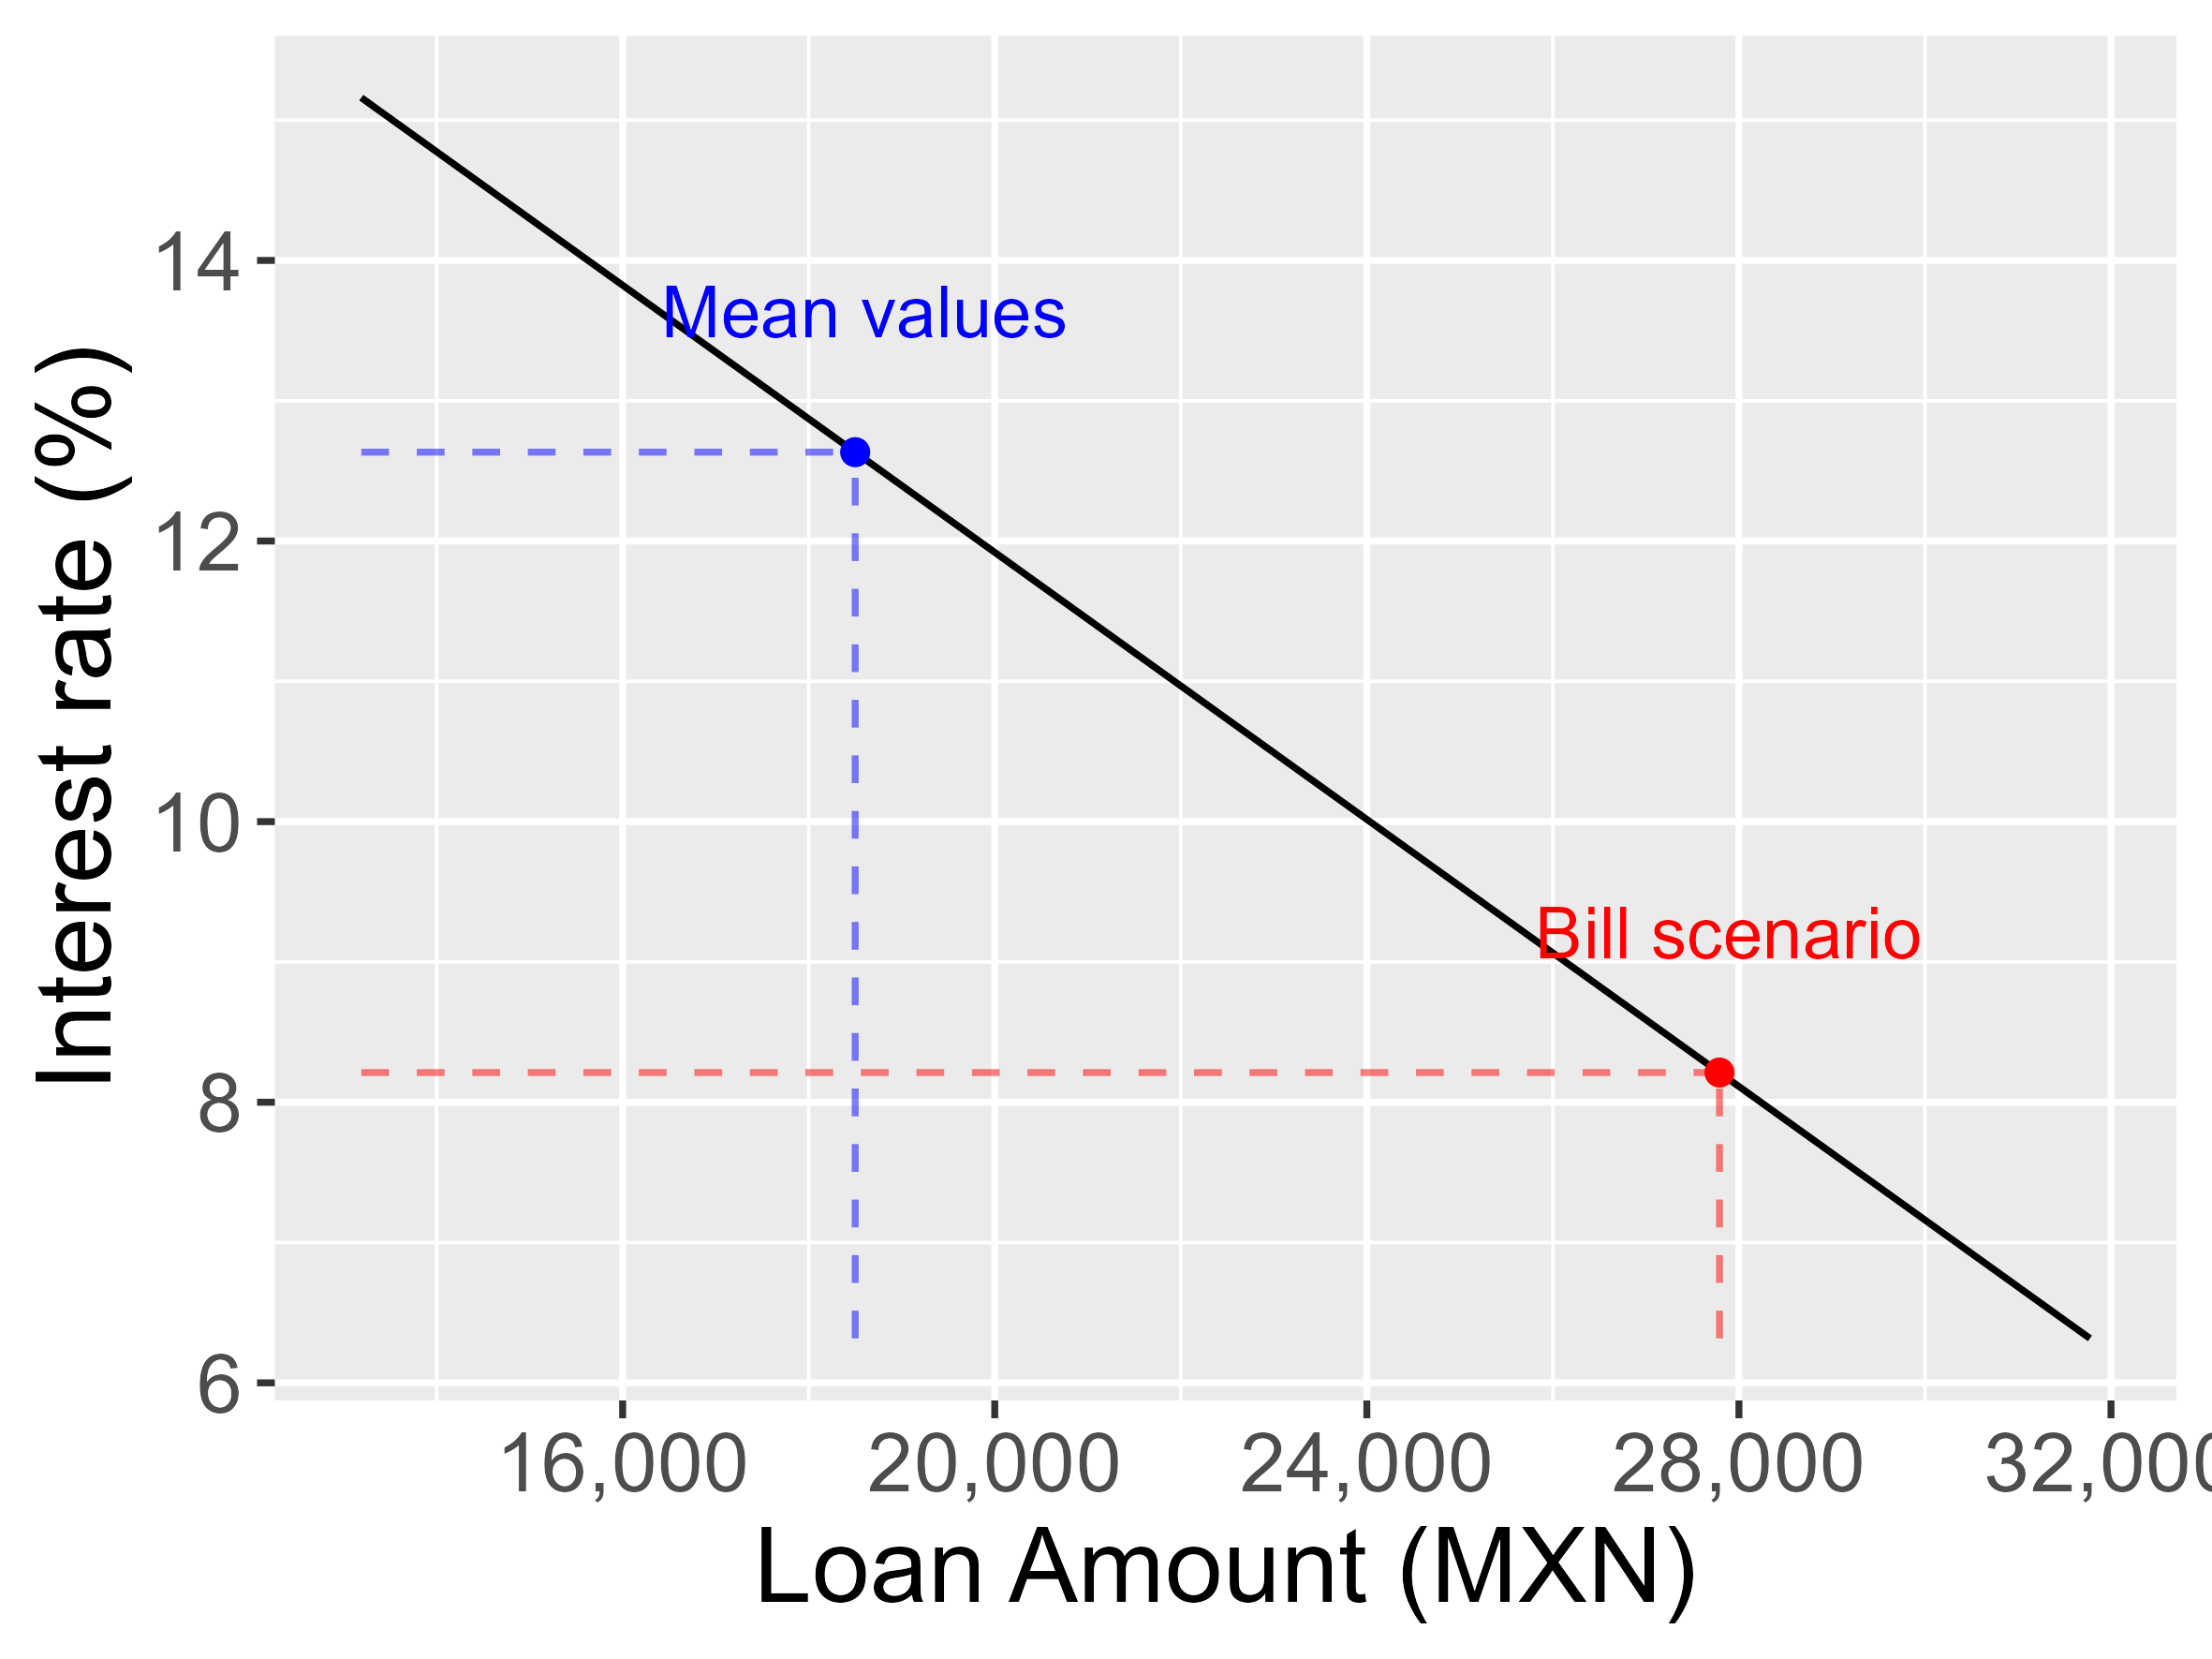
\includegraphics[scale=.75]{Imagenes/Demand.png}
\caption{Demand curve for credit.}
\fnote{ \textit{Note:} A decrease in the interest rate, from 12.6\% to 8.15\%, leads to an increase in the average loan amount by industry, from 23,392 to 66,845 thousand MXN.}
\label{Fig_Demand}
\end{center}
\end{figure}

I find the demand for credit in the Mexican market to be elastic, $-1.66$. This suggests that a regulatory measure aimed at reducing the interest rate would likely lead to a substantial increase in the average loan amount extended to borrowers. Note that,  such a scenario could have potential repercussions for the banking sector

Under these circumstances, banks are likely to face a higher exposure to default risk, and, consequently, loss given default. Thus, despite we are assuming G7 banks can increase their supply limitless, the rise in expected loss could derive into more stringent underwriting criteria to mitigate large losses. That is, to counter these surge in loan volumes, banks could impose additional requirements like better credit scores or requiring (additional) collateral to guarantee future repayment. As a result, credit may be reduced in general and the reform would have opposite results to those expected. 

Such a scenario reflects a shift from price rationing to equilibrium quantity rationing, as suggested by \citep[p. 4]{blundell1992credit}. This transition implies that the equilibrium quantity of credit demanded and supplied would be adjusted to achieve a balance in the market, in contrast to the traditional price-based allocation. 

An alternative policy that does not distort prices is recommended. For example, by providing collateral by the government, in the form of recommendation, to those companies in compliance with fiscal burdens such as taxes and social security obligations, which would enhance their credit profile and reduce their interest rates. 

The model inhere does not account for all the potential outcomes of the bill derived from asymmetric information issues. One main concern, for instance, is the presence of adverse selection in the financial markets. This phenomenon occurs when borrowers that see high interest rate as unfavourable do not ask for credit, resulting in a situation where a decrease in interest rates could attract a larger number of borrowers, which in the end would imply a riskier pool of borrowers.

To address such complexities, a structural model, like the one presented in \cite{crawford2018asymmetric} would be more appropriate to capture such effect. In their research, they examine the correlation between the unobserved determinants of demand for credit and default and interpret this as adverse selection. They find a statistically significant correlation coefficient of 0.16, which implies that firms with a higher unexplained propensity to borrow, on both the extensive and intensive margins, are also more likely to default. 


\chapter{Conclusions} \label{sect6}

I estimated interest rate elasticities that evidence an elastic credit demand curve using a reduced-form demand model for Mexican SMEs. The model allows me to disentangle the effects of interest rate and term-to-maturity on the loan amount. 

These findings have several important policy implications. I used the results to analyze possible regulatory policies in the credit sector. I find evidence that such a price distortion policy may possibly reduce credit in case a reform oriented to decrease interest rates is carried out, contrary to the expected results. Thus, the results of this research are of interest to policymakers, who can then make more informed interventions.

In light of these potential outcomes, any regulatory reform aimed to manipulate interest rates in the credit market should be approached with caution. While a decrease in interest rates might seemingly boost loan amounts, it may also trigger other events leading to tightened credit conditions and an overall reduction in credit accessibility. As such, a comprehensive analysis of the potential consequences and the interplay of various factors should be undertaken before implementing any policy adjustments.

A comprehensive analysis is crucial for policymakers, who should not to disregard the potential consequences of asymmetric information in the credit market. By incorporating these effects into the model would provide a more accurate understanding of the bill's effects on the credit market. 

 
Further research in this area could explore additional topics that can significantly enhance our understanding of credit dynamics and the implications of asymmetric information in the financial markets. 

One potential avenue for investigation is further exploiting CNBV'S information. On one side there is banks' operational information (number of staff, branches, ATM's, etc.) which can be used to estimate the credit supply. By leveraging the operational data of banks, one can gain valuable insights into the factors influencing banks' costs. Analyzing this data could shed light on how banks respond to changes in firms' demand for credit, incumbent economic conditions, previous regulatory policies, and other relevant factors. 

Moreover, the development of a structural model that incorporates default rates, which were not considered in the current study, is another relevant topic for further exploration. Understanding the relationship between default rates and the underlying asymmetric information issues is of relevance to disentangling the intricate relationships of credit markets and can shed light on the overall stability of the financial system.

In addition to the current scope of this research, it is of interest to extend the analysis to encompass large firms and the remaining banks not previously considered. These groups may exhibit distinctive credit behavior due to their unique characteristics and financial profiles. By extrapolating the results to include a more diverse sample of borrowers and lenders, researchers can identify potential variations in credit supply dynamics and better understand how the proposed bill might affect different segments of the market.

Overall, delving into these further research topics will significantly contribute to the understanding of credit supply mechanisms, asymmetric information issues, and the implications of potential policy changes. A comprehensive examination of banks' operational data, incorporation of default rate information, and the consideration of a broader set of firms and lenders will provide valuable insights that can inform policymakers and contribute to the advancement of financial regulations and practices.



%----------------------------------------------------------------------------------------
%	APÉNDICES
%----------------------------------------------------------------------------------------

%\begin{appendix}
%
%\chapter{Cuadros anexos}

\noindent 
%
%\end{appendix}

%----------------------------------------------------------------------------------------
%	BIBLIOGRAFÍA
%----------------------------------------------------------------------------------------


%\chapter*{References}
\cleardoublepage
\phantomsection
\addcontentsline{toc}{chapter}{References}

\renewcommand\bibname {References}

\bibliographystyle{apalike}
\bibliography{Referencias/References}


% Macro. Esto es muy importante, no lo borren

%\makeatletter
%\renewenvironment{thebibliography}[1]
%     {\@mkboth{\MakeUppercase\refname}{\MakeUppercase\refname}%
%      \list{}%
%           {\setlength{\labelwidth}{0pt}%
%            \setlength{\labelsep}{0pt}%
%            \setlength{\leftmargin}{\parindent}%
%            \setlength{\itemindent}{-\parindent}%
%            \@openbib@code
%            \usecounter{enumiv}}%
%      \sloppy
%      \clubpenalty4000
%      \@clubpenalty \clubpenalty
%      \widowpenalty4000%
%      \sfcode`\.\@m}
%     {\def\@noitemerr
%       {\@latex@warning{Empty `thebibliography' environment}}%
%      \endlist}
%\makeatother
%
%\begin{thebibliography}{111}
%
%% Lista
%
%% La manera recomendada para citar papers o libros en el formato de Chicago esta en el siguiente vínculo: https://www.chicagomanualofstyle.org/tools_citationguide/citation-guide-2.html
%
%% Es importante poner el apellido del autor seguido del año de publicación, una coma y las páginas consultadas en el texto antes de puntuar y entre paréntesis para las citas en el cuerpo de la tesis
%
%% Ejemplo:
%
%% Las \textit{causas próximas} del crecimiento son conocidas: tecnología, capital humano y físico. La pregunta es ¿por qué unos países sí tienen estas causas próximas y otros no? La respuesta son las \textit{causas fundamentales:} suerte, geografía, cultura e instituciones (Acemoglu 2009, 110).
%
%%AAAAA
%%\bibitem{abram57} Abramovitz, Moses. 1957. «Resources on Output Trends in the United States since 1870.» \textit{The American Economic Review} 46 (2): 5–23.
%%
%%\bibitem{acemoglu09} Acemoglu, Daron. 2009. \textit{Introduction to Modern Economic Growth.} Princeton: Princeton University Press.
%
%%BBBBB
%
%%CCCCC
%
%%DDDDD
%
%%EEEEE
%
%%FFFFF
%
%%GGGGG
%
%%HHHHH
%
%%IIIII
%
%%JJJJJ
%
%%KKKKK
%
%%LLLLL
%
%%MMMMM
%
%%NNNNN
%
%%OOOOO
%
%%PPPPP
%
%%QQQQQ
%
%%RRRRR
%
%%SSSSS
%
%%TTTTT
%
%%UUUUU
%
%%VVVVV
%
%%WWWWW
%
%%XXXXX
%
%%YYYYY
%
%%ZZZZZ
%
%\end{thebibliography}

\newpage
\thispagestyle{empty}
\begin{table}[p]
\centering
\small
\label{ed}
\begin{tabular}{c}
\textit{La elasticidad de la tasa de interés de la demanda de crédito:} \\ \textit{evidencia empírica de empresas mexicanas.}\\ escrito por Jesús López,\\ se terminó de imprimir en agosto de 2023\\ en los talleres de Tesis Matozo.\\ Campeche 156, colonia Roma,\\ Ciudad de México.
\end{tabular}
\end{table}

% Si lo prefieren, avisen a su taller que esta página ya la incluyeron ustedes para que no les impriman las que ellos usan. Lo recomiendo ampliamente

%%%%%%%%%%%%%%%%%%%%%%%%%%%%%%%%%%%%%%%%%%%%%%%%%%%%%%%%%%%%%%%%%%%%%%%%%%%%%%%%%%%%%%%

\end{document}